\documentclass[a4paper,12pt]{book}     
\usepackage[utf8]{inputenc} 
\usepackage[T1]{fontenc}
\usepackage{times}
\usepackage{graphicx}
\usepackage{anysize}
\usepackage{enumerate}
\usepackage{color} 
\usepackage{tikz}
\marginsize{.5cm}{.5cm}{.5cm}{2.5cm}

\begin{document}
\begin{figure}[!htb]
	\centering
	\begin{tikzpicture}
	\node at (0,0) {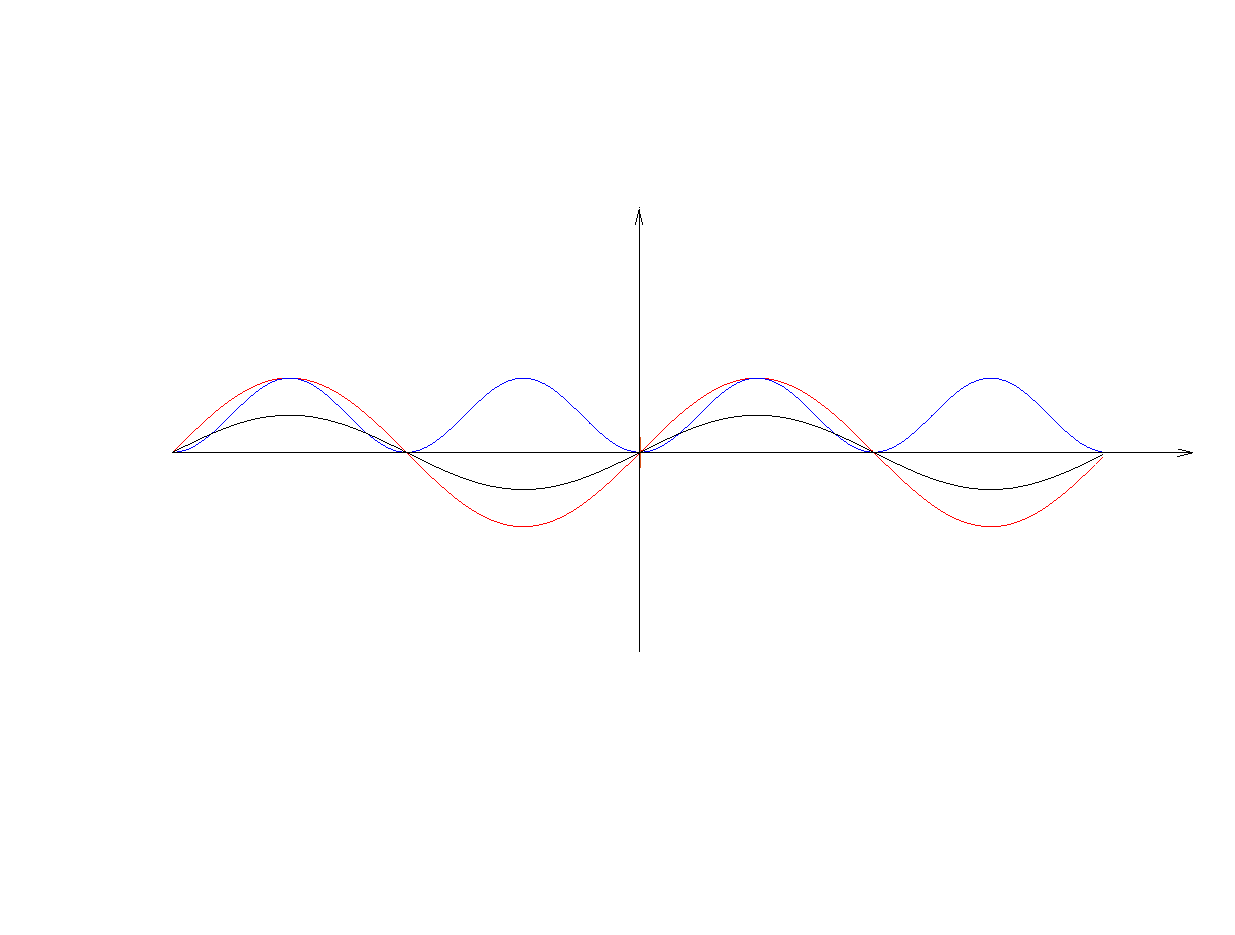
\includegraphics[scale=1]{f1b}};
	\node at (6.7,-1.3) {$f(x) = \sin(x)$};
	\node at (6.7,1.8) {$g(x) = \sin^2(x)$};
	\node at (2.28,0.5) {$h(x) = \frac{\sin(x)}{2}$};
	\end{tikzpicture}
	\caption{Wykresy funkcji}
	\label{fig:funkcje}
\end{figure}
\end{document}